\documentclass[11pt]{scrartcl}

\usepackage[utf8]{inputenc}
\usepackage{amsmath}
\usepackage{biblatex}
\usepackage{caption}
\usepackage{float}
\usepackage{graphicx}
\usepackage{subcaption}

\renewcommand{\bibfont}{\footnotesize}
%\pagenumbering{gobble}
\usepackage{hyperref}
\addbibresource{report.bib}

\title{Phases in Context Tree Weighting}
\subtitle{CS281B: Final Project Report}
\author{Constantin Berzan (joint work with Eric Tzeng)\footnote{We are grateful
to Wouter M. Koolen for discussion and useful ideas.}}
\date{May 1, 2014}

\begin{document}
\maketitle

\begin{abstract}
The official implementation of the context tree weighting (CTW) algorithm uses
a complicated notion of {\em phases} to organize the context trees, providing
little justification for it. In an attempt to uncover the underlying reasons
for using phases, we implemented and experimented with several variations of
the CTW algorithm. This document reports our experiments and results.
\end{abstract}

%%%%%%%%%%%%%%%%%%%%%%%%%%%%%%%%%%%%%%%%%%%%%%%%%%%%%%%%%%%%%%%%%%%%%%%%%%%%%%
\section{Introduction}
\label{sec:intro}

Shannon's source coding theorem tells us that a symbol $x$ can be encoded in
$-\log_2(P(x))$ bits, where $P(x)$ is the probability assigned to symbol $x$ by
some model. Thus, the higher the probability $P(x)$, the more compression we
can achieve. Suppose we are trying to compress a bit sequence $x_{1:T}$. We can
see this sequence as a single symbol $x$, taken from an alphabet of all
possible binary sequences of length $T$. Then, our model needs to assign a
probability to every sequence of bits, such that the total probability for all
possible sequences of length $T$ sums to 1.

Context tree weighting (CTW) is one such probabilistic model that achieves good
compression performance, and also lends itself to theoretical analysis.
\textcite{eidma} present the context tree weighting algorithm as operating on a
sequence of bits. However, their implementation uses a more complicated
construction. They have an ensemble of 255 context trees, with whole bytes as
context, and for every bit, they choose the context tree based on the previous
bits in the same byte. The CTW authors claim\footnote{{\tt
http://www.ele.tue.nl/ctw/overview/structure.html}} that ``it appeared to be a
better choice'' to use phases, but they do not provide any insight into why
this may be the case.

Our goal was to understand why CTW with phases does better than the simpler
binary CTW, or an extension of the binary CTW that predicts whole bytes at a
time. We implemented these three varieties of the CTW algorithm, and
investigated their compression performance given various kinds of data. Our
implementation and experiments are available at {\tt
https://github.com/cberzan/ctw}.

The rest of this document is organized as follows: Sections
\ref{sec:wct-binary}, \ref{sec:wct-phases}, and \ref{sec:wct-bytes} present the
context tree varieties that we implemented. Section \ref{sec:transformations}
presents two text transformations that we devised for investigating which
properties of ASCII the algorithm takes advantage of. Section \ref{sec:results}
discusses our results, and section \ref{sec:conclusion} states our conclusions
and ideas for future work.


%%%%%%%%%%%%%%%%%%%%%%%%%%%%%%%%%%%%%%%%%%%%%%%%%%%%%%%%%%%%%%%%%%%%%%%%%%%%%%
\section{The Binary Weighted Context Tree (WCTBinary)}
\label{sec:wct-binary}

The Binary Weighted Context Tree (WCTBinary) is a complete binary tree of a
pre-specified depth. Each node $s$ represents a context, which is a sequence of
bits. If the node $s$ is a leaf, then it has no children. Otherwise, the node
$s$ has two children, $0s$ and $1s$, obtained by prepending an additional bit
of context.  We use $\lambda$ to denote the root node, which represents an
empty context.

In the implementation, we only allocate memory for the nodes that correspond to
contexts that have been seen at least once. Each node stores four values: $a$,
$b$, $P_e$, and $P_w$. We use a superscript to denote which node we are
referring to. $a$ and $b$ are the number of zero and one bits seen in the
node's context. $P_e$ is the probability given by the KT estimator for $a$ and
$b$, i.e. $P_e^s = P_{KT}(a^s, b^s)$. $P_{KT}$ is given by the following
recurrence:

\begin{align*}
P_{KT}(0, 0)   &= 1 \\
P_{KT}(a, b+1) &= P_{KT}(a, b) \frac{b + 1/2}{a + b + 1} \\
P_{KT}(a+1, b) &= P_{KT}(a, b) \frac{a + 1/2}{a + b + 1}
\end{align*}
\
$P_w$ is a weighting of the probability at this node and the probability at the
children:

\[
P_w^s =
\left\{
\begin{array}{ll}
\frac{1}{2} P_e^s + \frac{1}{2} P_w^{0s} P_w^{1s}
    & \mbox{if $s$ is not a leaf} \\
\phantom{\frac{1}{2}} P_e^s
    & \mbox{if $s$ is a leaf}
\end{array}
\right.
\]

The best way to grasp context trees is by example. Figure \ref{fig:bin-tree}
shows the example tree from \textcite{eidma}. This tree was constructed from
the sequence $x_{1:T} = 0110100$, with initial context $...010$ and a depth of
3.  The circled node represents context $s = 10$, and has two children: $0s =
010$ and $1s = 110$. The circled node has $a = 2$ and $b = 1$, meaning that we
have seen the sequence $s0 = 100$ two times, and the sequence $s1 = 101$ one
time.

\begin{figure}[h!]
    \centering
    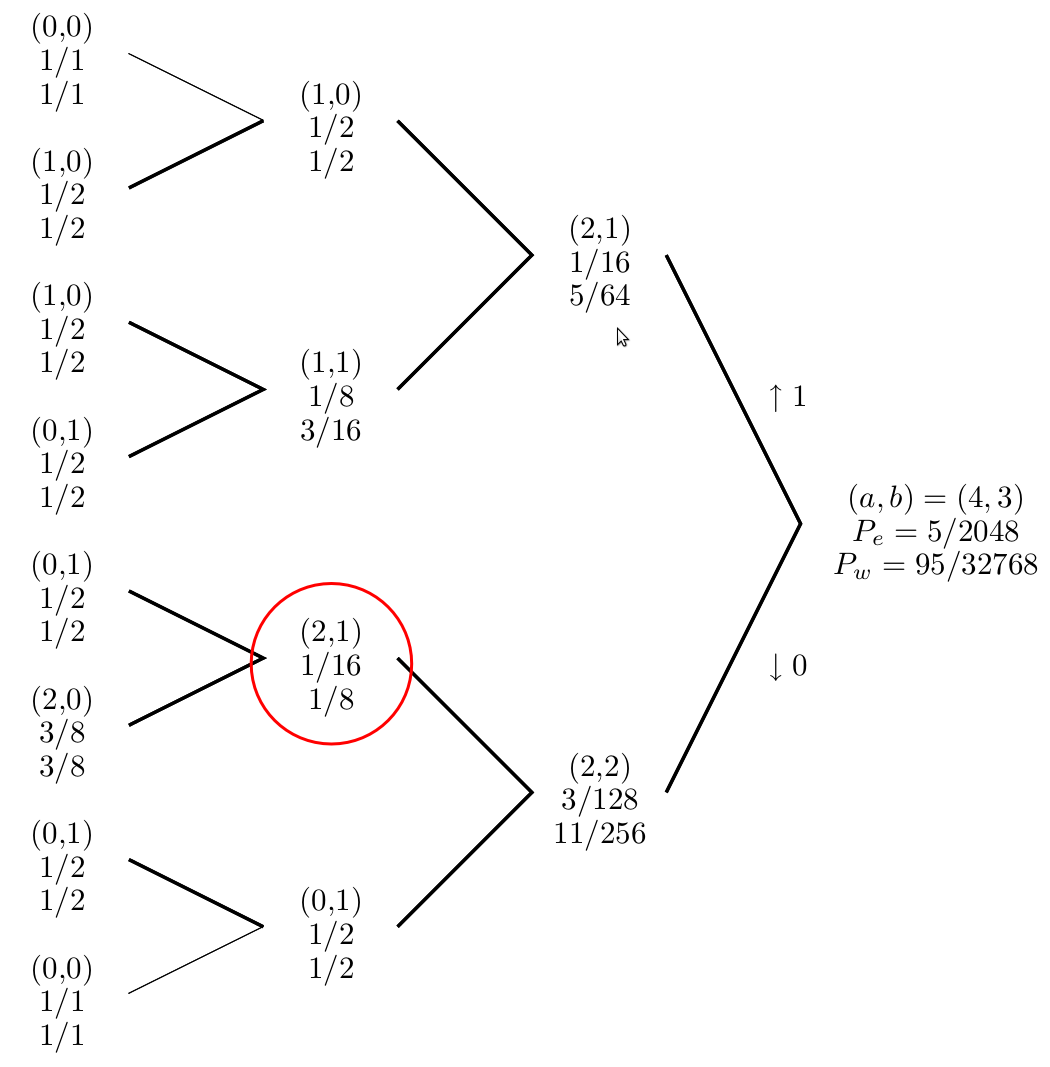
\includegraphics[width=12cm]{eidma-fig-3-2-ed.png}
    \caption{Example binary weighted context tree from \textcite{eidma}.}
    \label{fig:bin-tree}
\end{figure}

How do we update this tree? Suppose the next symbol is $x_{T+1} = 0$. The
context is $x_{T-2:T} = 100$. We simply locate the leaf node $100$, increment
$a$ because we saw a zero, and update $P_e$ and $P_w$ according to their
definitions. We then update $a$, $b$, $P_e$, and $P_w$ for all the nodes on the
path from the leaf node to the root.

How do we use this tree for compression? At any point, the root weighted
probability $P_w^\lambda$ represents the probability that the tree assigns to
the sequence of bits seen so far, i.e. $P(x_{1:t})$. For the encoder, we need
the conditional probability that the next bit is a zero:
$P(x_{t+1} = 0 | x_{1:t})$. (The probability that the next bit is a one is just
$P(x_{t+1} = 1 | x_{1:t}) = 1 - P(x_{t+1} = 0 | x_{1:t})$.)
To obtain this conditional probability, we do a
``dummy 0 update'' to get $P(x_{1:t}, x_{t+1} = 0)$, and then compute
\[
P(x_{t+1} = 0 | x_{1:t}) = \frac{ P(x_{1:t}, x_{t+1} = 0) }{ P(x_{1:t}) }.
\]
A ``dummy 0 update'' means that we traverse the tree and update $P_w^\lambda$
as if seeing that the next bit is a zero, but without actually making any
changes to the tree. Figure \ref{fig:enc-dec} shows the top-level encoding and
decoding loops in pseudocode. Since the tree receives the same sequence of
updates during encoding and decoding, the sequence of probabilities sent to the
encoder and decoder is consistent.

\begin{figure}[h!]
    \centering
    \begin{subfigure}[b]{0.5\textwidth}
\begin{verbatim}
def encode(data, max_depth):
    tree = WCTBinary(max_depth)
    encoder = ArithmeticEncoder()
    context = [0, 0, ..., 0]
    for bit in data:
        p0 = tree.get_p0(context)
        encoder.encode_bit(p0, bit)
        tree.update(context, bit)
        context = context[1:] + [bit]
    encoder.finalize() \end{verbatim}
        \caption{Encoding}
    \end{subfigure}
    ~
    \begin{subfigure}[b]{0.45\textwidth}
\begin{verbatim}
def decode(enc_data, max_depth):
    tree = WCTBinary(max_depth)
    decoder = ArithmeticDecoder(enc_data)
    context = [0, 0, ..., 0]
    for i in range(msg_len):
        p0 = tree.get_p0(context)
        bit = decoder.decode_bit(p0)
        tree.update(context, bit)
        context = context[1:] + [bit]
    decoder.finalize() \end{verbatim}
        \caption{Decoding}
    \end{subfigure}
    \caption{Pseudocode for encoding and decoding.}
    \label{fig:enc-dec}
\end{figure}

% TODO: talk about the probability of the whole sequence?


%%%%%%%%%%%%%%%%%%%%%%%%%%%%%%%%%%%%%%%%%%%%%%%%%%%%%%%%%%%%%%%%%%%%%%%%%%%%%%
\section{The Weighted Context Tree with Phases (WCTPhases)}
\label{sec:wct-phases}

The Weighted Context Tree with Phases (WCTPhases) is an ensemble of context
trees. We have a total of $1 + 2 + ... + 128 = 255$ trees, one corresponding to
each possible prefix within a byte. Let $x_{i,j}$ denote the j-th bit of the
i-th byte of the input sequence.  When processing $x_{i,j}$, we select the tree
corresponding to the previous bits in the current byte: $x_{i,1}, ...,
x_{i,j-1}$. The context now consists of the previous {\em bytes}, so all the
trees are 256-ary, not binary. But each tree still predicts only the
probability of the next bit. Each node stores $a$, $b$, $P_e$, and $P_w$, as
before, except that $P_w$ is now computed as

\[
P_w^s =
\left\{
\begin{array}{ll}
\frac{1}{2} P_e^s + \frac{1}{2} \prod_{i=0}^{255}{ P_w^{i,s} }
    & \mbox{if $s$ is not a leaf} \\
\phantom{\frac{1}{2}} P_e^s
    & \mbox{if $s$ is a leaf}
\end{array}
\right.
\]

Since we have 255 trees instead of one, it is no longer obvious what the
probability of the whole sequence is. It turns out that this probability is
just the product of $P_w$ values at the root of every tree:
\[
P(x_{1:T}) = \prod_{n=1}^{255} P_{w, n}^\lambda
\]
where $n$ ranges over all trees (the empty prefix, then the prefixes $0$ and
$1$, then the prefixes $00$, $01$, $10$, $11$, then all prefixes of length 3,
and so on). This fact can be seen by writing out the probability of the whole
sequence as a product of conditional probabilities, and factoring the
conditional probabilities according to the tree that they contribute to.


%%%%%%%%%%%%%%%%%%%%%%%%%%%%%%%%%%%%%%%%%%%%%%%%%%%%%%%%%%%%%%%%%%%%%%%%%%%%%%
\section{The Weighted Context Tree on Bytes (WCTBytes)}
\label{sec:wct-bytes}

The Weighted Context Tree on Bytes (WCTBytes) is a straightforward extension of
WCTBinary to bytes. In particular, the context is now a sequence of bytes, not
bits, and the tree now predicts the next byte, not the next bit. Each node
stores the symbol counts $n_0, ..., n_{255}$, and the probabilities $P_e$ and
$P_w$. $P_w$ is computed in the same way as in WCTPhases. $P_e$ is an
extension of KT to 256 symbols:
\[
P_e(n_0, ..., n_i + 1, ..., n_{256}) =
P_e(n_0, ..., n_i, ..., n_{256})
\frac{ n_i + 1/2 }{ n_0 + ... + n_{256} + 128 }.
\]

Using WCTBytes for compression requires a more complicated arithmetic encoder:
one that encodes one byte at a time, rather than one bit at a time. But to
evaluate the compression ratio of WCTBytes we do not need to implement this
encoder. We only need to know $P_w^\lambda$, since by Shannon's theorem, the
length of the encoded (compressed) string will be $-\log_2(P_w^\lambda)$ bits.


%%%%%%%%%%%%%%%%%%%%%%%%%%%%%%%%%%%%%%%%%%%%%%%%%%%%%%%%%%%%%%%%%%%%%%%%%%%%%%
\section{Plaintext Transformations}
\label{sec:transformations}

English text represented in ASCII exhibits two properties that might be
exploited by a compression algorithm: locality and byte alignment. Locality
means that commonly used characters have similar representations (the
lower-case letters range from {\tt 01100001} to {\tt 01111010}, and the
upper-case letters range from {\tt 01000001} to {\tt 01011010}). Byte alignment
means that each character is represented as exactly one byte.

To investigate how much our compression algorithms rely on these properties, we
devised two simple transformations that disrupt these properties. The {\bf
scrambling} transformation passes the text through a random 1-1 mapping from
bytes to bytes, thus disrupting locality. The {\bf misaligning} transformation
prepends a zero bit to every byte, thus making each character occupy nine bits,
and disrupting byte alignment. Figure \ref{fig:transformations} summarizes
these transformations in pseudocode.

\begin{figure}[h!]
    \centering
    \begin{subfigure}[b]{0.45\textwidth}
\begin{verbatim}
def scramble(input):
    mapping = rand_permut(256)
    for char in input:
        output mapping[char] \end{verbatim}
        \caption{Scrambling transformation}
    \end{subfigure}
    ~
    \begin{subfigure}[b]{0.45\textwidth}
\begin{verbatim}
def misalign(input):
    for byte in input:
        output 0
        output all bits of byte \end{verbatim}
        \caption{Misaligning transformation}
    \end{subfigure}
    \caption{Pseudocode for the plaintext transformations.}
    \label{fig:transformations}
\end{figure}



%%%%%%%%%%%%%%%%%%%%%%%%%%%%%%%%%%%%%%%%%%%%%%%%%%%%%%%%%%%%%%%%%%%%%%%%%%%%%%
\section{Results and Discussion}
\label{sec:results}

We ran experiments on an English text document of 1270 characters. (It is the
first paragraph from Harlan Ellison's short story, {\em ``Repent, Harlequin!''
Said the Ticktockman}, which is in turn a quotation from Henry David Thoreau's
essay, {\em Civil Disobedience}.)

We validated our implementation in two ways: First, we verified that encoding
and then decoding the text produced the original text back. Second, we verified
that our implementation of WCTPhases obtained the same compression ratio as the
official CTW implementation run with the KT estimator. Thus, we are confident
that our implementation of WCTPhases is equivalent to the official CTW
implementation.

Our implementation was not nearly as fast as the official CTW implementation.
Encoding and decoding our example text took 5.8 seconds with WCTBinary, and
21.5 seconds with WCTPhases. The official CTW implementation took 0.05 seconds
for the same task (430 times faster than WCTPhases). These runtimes are
reported for a modern laptop with a 2.9 GHz CPU. The official CTW
implementation is written in C and includes multiple optimizations for speed
(single-path pruning, pre-computed logarithm tables, and a more advanced
arithmetic encoder). In our Python implementation, we focused on simplicity and
easy experimentation, rather than speed.

For our main experiment, we compared the compression ratio obtained by
WCTBinary, WCTPhases, and WCTBytes on the original text, a scrambled version of
the original text, and a misaligned version of the original text. All trees
were configured with a depth of 6 bytes, or 48 bits, which is the default value
used in the official CTW implementation. Table \ref{tab:results} summarizes our
results.

\begin{table}[h!]
    \centering
    \begin{tabular}{l|lll}
        & plain text & scrambled text & misaligned text \\
        \hline
        WCTBinary & 4.69 bits/byte & 5.41 bits/byte & 4.64 bits/byte \\
        WCTPhases & 3.90 bits/byte & 4.12 bits/byte & 6.87 bits/byte \\
        WCTBytes  & 4.61 bits/byte & 4.61 bits/byte & 7.45 bits/byte \\
    \end{tabular}
    \caption{Compression ratio for the various algorithms and plaintext
    transformations.}
    \label{tab:results}
\end{table}

WCTBinary did equally well for the plain text and the misaligned text, but it
did poorly on the scrambled text. This tells us that WCTBinary takes advantage
of the locality of ASCII, but does not take advantage of byte-aligned data.

WCTPhases did comparably well for the plain text and the scrambled text, but it
did much worse on the misaligned text. This tells us that WCTPhases does not
rely on locality as much, but it does rely heavily on byte-aligned data.

WCTBytes was unaffected by scrambling at all, but it did much worse on
misaligned text. This was to be expected, since out of all three methods,
WCTBytes is the most reliant on byte-aligned data.

We verified that the results we just presented hold for other English text
documents of similar length. For longer documents, the compression ratios are
better, but the effect of scrambling and misalignment remain qualitatively the
same.


%%%%%%%%%%%%%%%%%%%%%%%%%%%%%%%%%%%%%%%%%%%%%%%%%%%%%%%%%%%%%%%%%%%%%%%%%%%%%%
\section{Conclusion and Future Work}
\label{sec:conclusion}

The official CTW documentation\footnote{{\tt
http://www.ele.tue.nl/ctw/overview/structure.html}} mentions that the binary
tree and the tree on bytes ``do not give the desirable results'', while the
tree with phases performs better. We have implemented all three varieties of
trees, and investigated their performance. Our experiments with scrambled and
misaligned text suggest that WCTPhases performs better than WCTBinary primarily
because the former takes advantage of byte alignment in ASCII data. WCTPhases
also performs better than WCTBytes, because each tree in WCTPhases predicts one
bit at a time, which requires less training data than predicting one byte at a
time, as in WCTBytes.

We started a few other experiments, whose results were not as clean-cut as the
ones we presented here. For example, we investigated the most-often visited
tree branches in WCTBinary, and observed the sequence ...0010000001... over and
over again. This sequence is composed of the ASCII character space (00100000)
followed by the first two bits of an ASCII lower-case or upper-case letter. We
also investigated the trees produced by WCTPhases, and found that some trees
were more skewed than others. For example, the tree for the phase 01... had a
high root $P_w$, predicting a 1 with high probability because lower-case
letters are far more common than upper-case letters. Other trees were less
certain about their prediction, and had lower root $P_w$ values. We also
experimented with changing the weighting factor away from 1/2, or making it
dependent on the depth within the tree, but we did not find any setting that
performed better than the default. Future work consists of doing more detective
work to understand other properties of text that the CTW algorithm might take
advantage of. It would also be interesting to adapt the algorithm to work well
with other kinds of data, such as images.


%%%%%%%%%%%%%%%%%%%%%%%%%%%%%%%%%%%%%%%%%%%%%%%%%%%%%%%%%%%%%%%%%%%%%%%%%%%%%%
\printbibliography


\end{document}
